\documentclass[aspectratio=169,11pt]{beamer}

\usetheme{metropolis}
\metroset{block=fill}

\usepackage[T1]{fontenc}
\usepackage[utf8]{inputenc}
\usepackage[brazil]{babel}
\usepackage{amsmath}
\usepackage{amssymb}
\usepackage{booktabs}
\usepackage{graphicx}
\usepackage{tikz}
\usetikzlibrary{arrows.meta}

\graphicspath{{figs/}}

% Símbolo esquemático de VANT (quadricóptero, vista lateral) para uso em cenas TikZ
\newcommand{\dronesym}{%
  \draw[line width=0.5pt] (-0.5,0)--(0.5,0);
  \fill[gray!55] (-0.13,-0.09) rectangle (0.13,0.09);
  \draw[line width=0.5pt,fill=gray!25] (-0.5,0) ellipse (0.19 and 0.05);
  \draw[line width=0.5pt,fill=gray!25] (0.5,0) ellipse (0.19 and 0.05);
}
% Sensor no solo com antena
\newcommand{\sensorsym}[1]{%
  \fill[blue!20] (#1-0.08,0) rectangle (#1+0.08,0.3);
  \draw[line width=0.4pt] (#1-0.08,0) rectangle (#1+0.08,0.3);
  \draw[line width=0.4pt] (#1,0.3)--(#1,0.46);
  \fill (#1,0.46) circle (0.03);
}

\title{Otimização do plano de voo de VANTs para coleta de dados de sensores IoT}
\subtitle{Projeto de Graduação em Computação}
\author{Lucas de Medeiros Santos}
\institute{Universidade Federal do ABC \\ Orientador: Prof. Dr.~Rodrigo Augusto Cardoso da Silva}
\date{Santo André, 2026}

\begin{document}

{
\begin{frame}[plain, noframenumbering]
  \centering
  \vspace*{0.1cm}
  
\includegraphics[height=1.55cm]{logo.png}\\[0.4cm]
  {\usebeamerfont{title}\usebeamercolor[fg]{title}\inserttitle\par}
  \vspace{0.2cm}
  {\usebeamerfont{subtitle}\usebeamercolor[fg]{subtitle}\insertsubtitle\par}
  \vspace{0.35cm}
  {\color{gray!60}\rule{0.9\textwidth}{0.4pt}}\\[0.35cm]
  {\usebeamerfont{author}\insertauthor\par}
  \vspace{0.1cm}
  {\usebeamerfont{date}\insertdate\par}
  \vspace{0.25cm}
  {\footnotesize\insertinstitute\par}
\end{frame}
}

\begin{frame}{O que são VANTs?}
  \begin{columns}[c]
    \begin{column}{0.58\textwidth}
      \small
      \begin{itemize}
        \item Veículos aéreos não tripulados (VANTs), ou drones.
        \item Dois tipos principais de propulsão:
          \begin{itemize}
            \item \textbf{Asa fixa:} maior autonomia e velocidade, mas não param no ar.
            \item \textbf{Asa rotativa} (multirrotor): conseguem \emph{pairar} (\emph{hover}) sobre um ponto.
          \end{itemize}
        \item Neste trabalho: asa rotativa (DJI Matrice 300 RTK e Parrot Anafi USA).
      \end{itemize}
    \end{column}
    \begin{column}{0.42\textwidth}
      \centering
      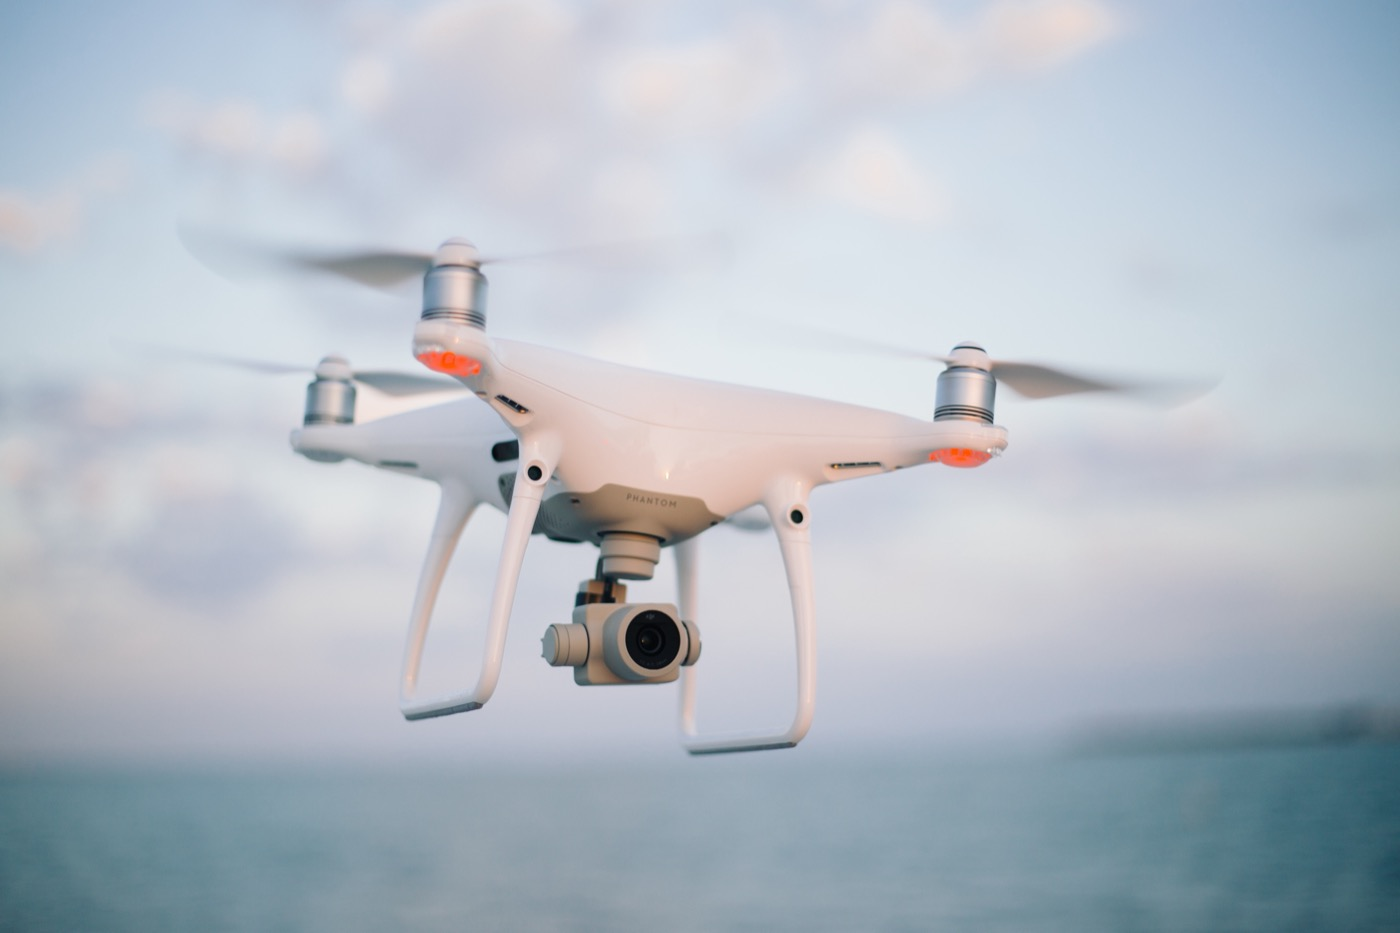
\includegraphics[width=\linewidth]{drone_generico.jpg}\\[2pt]
      {\tiny Foto: Josh Sorenson, CC0 (Wikimedia Commons).}
    \end{column}
  \end{columns}
\end{frame}

\begin{frame}{O que é IoT?}
  \begin{itemize}
    \item \textbf{Internet das Coisas (IoT):} objetos físicos conectados que coletam e transmitem dados do ambiente.
    \item \textbf{Redes de sensores sem fio (WSN):} nós de baixo consumo, distribuídos em uma área, que medem grandezas físicas e as enviam a um ponto de coleta.
    \item Sem infraestrutura de rede fixa, levar esses dados ao ponto de coleta é um desafio.
  \end{itemize}
  \vspace{0.5em}
  \centering
  \begin{tikzpicture}
    \draw[gray!45,line width=0.4pt] (0,0)--(8,0);
    \node[draw,fill=orange!25,minimum size=6mm,font=\scriptsize] at (0.4,0.32) {};
    \node[font=\scriptsize,anchor=west] at (0.8,0.32) {ponto de coleta};
    \foreach \x in {4.2,5.2,6.2,7.2,7.9}{ \sensorsym{\x} }
    \node[font=\scriptsize] at (6.0,-0.4) {sensores distribuídos};
  \end{tikzpicture}
\end{frame}

\begin{frame}{Aplicações no mundo real}
  VANTs coletam dados de sensores onde a infraestrutura fixa é limitada ou inexistente:
  \begin{itemize}
    \item \textbf{Agricultura de precisão:} sensores de solo e monitoramento de lavouras.
    \item \textbf{Monitoramento ambiental remoto:} sensores e boias em áreas sem cobertura de rede.
    \item \textbf{Resposta a desastres:} coleta contornando a infraestrutura danificada.
  \end{itemize}
  \vspace{0.4em}
  A seguir, um caso em destaque.
\end{frame}

\begin{frame}{Destaque: agricultura de precisão}
  \begin{columns}[c]
    \begin{column}{0.54\textwidth}
      \centering
      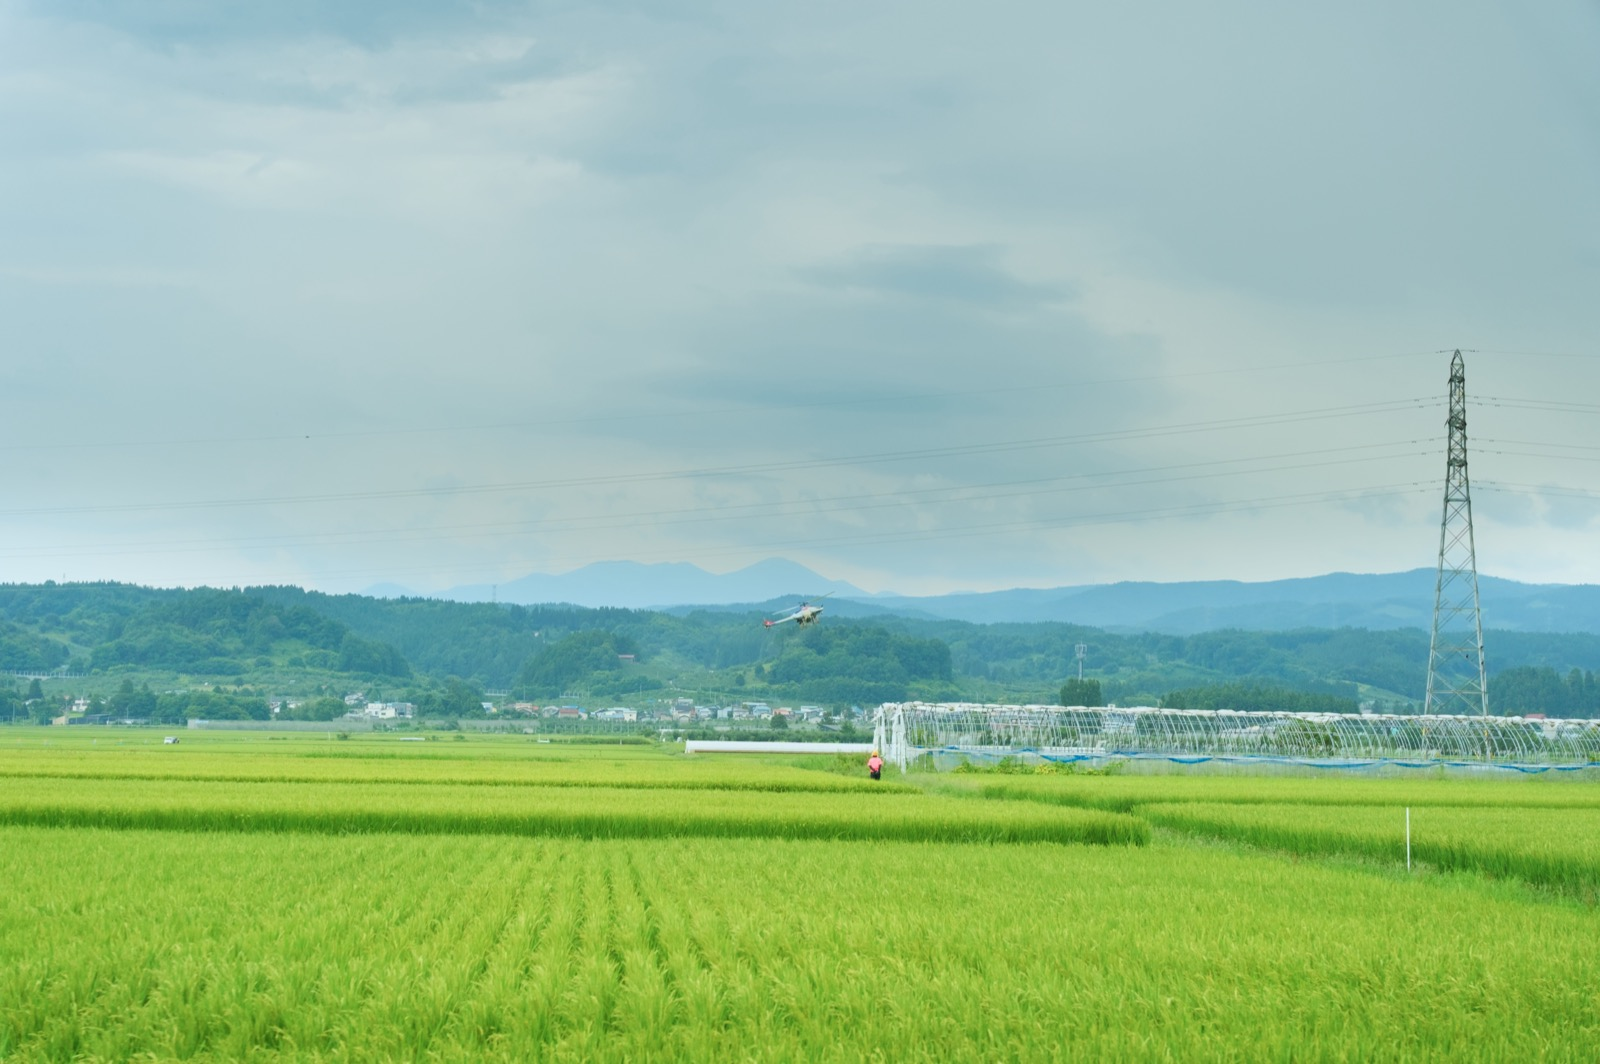
\includegraphics[width=\linewidth]{drone_agricola.jpg}\\[2pt]
      {\tiny Drone agrícola em arrozal (Aomori, Japão). Foto: Benlisquare, Wikimedia Commons, CC BY-SA 4.0.}
    \end{column}
    \begin{column}{0.46\textwidth}
      \small
      \begin{itemize}
        \item Sensores de solo medem umidade, pH e temperatura.
        \item O VANT coleta esses dados e complementa com sensoriamento aéreo.
        \item Plataformas autônomas já operam em campo.
      \end{itemize}
    \end{column}
  \end{columns}
\end{frame}

\begin{frame}{Do cenário real ao problema}
  \begin{columns}[c]
    \begin{column}{0.6\textwidth}
      \small
      \begin{itemize}
        \item Fio comum: sensores distribuídos, sem infraestrutura fixa, e um VANT como coletor móvel.
        \item Qualidade medida pela \emph{Age of Information} (AoI): idade do dado mais recente. Dados desatualizados perdem valor.
        \item O VANT tem energia (bateria) limitada.
        \item \textbf{Tensão central:} coletar mais informação {\itshape versus} gastar menos energia.
      \end{itemize}
    \end{column}
    \begin{column}{0.4\textwidth}
      \centering
      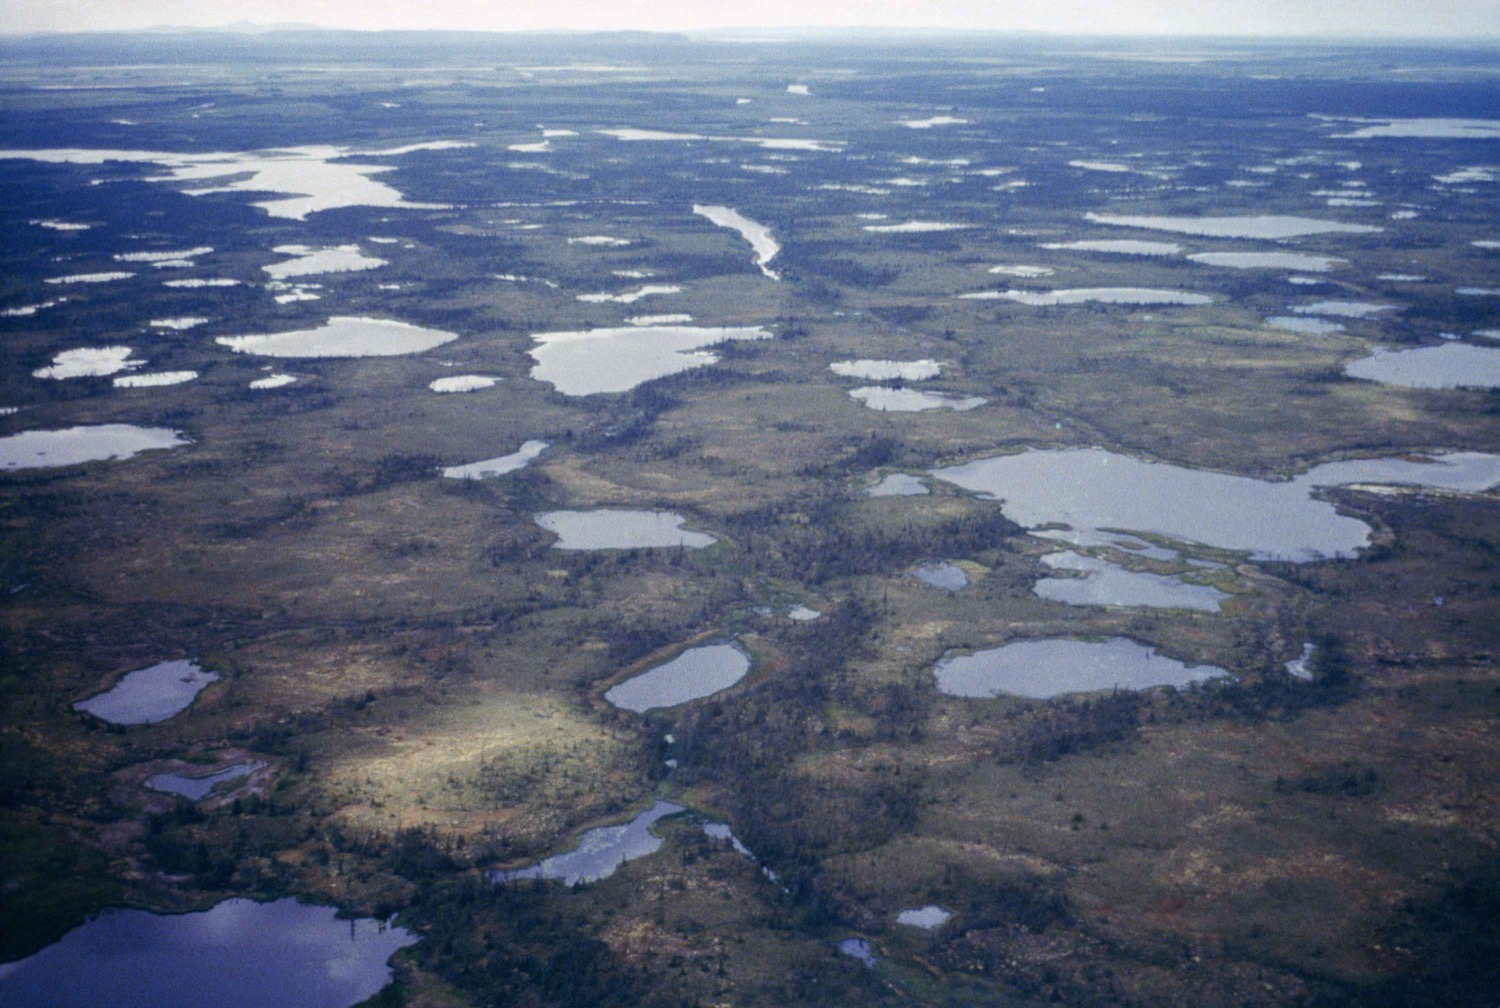
\includegraphics[width=\linewidth]{monitoramento_ambiental.jpg}\\[2pt]
      {\tiny Área alagada, monitoramento ambiental remoto. Foto: U.S. Fish and Wildlife Service, domínio público.}
    \end{column}
  \end{columns}
\end{frame}

\begin{frame}{O cenário considerado}
  \begin{itemize}
    \item Planejar a trajetória de um VANT: sair da base, coletar dados dos sensores e retornar.
    \item Dois objetivos conflitantes:
      \begin{itemize}
        \item maximizar a AoI coletada (priorizar dados mais antigos),
        \item minimizar a energia consumida.
      \end{itemize}
    \item Coleta por \emph{hovering}: pairar sobre o sensor durante um \emph{slot}.
    \item Cada sensor é visitado no máximo uma vez por missão.
    \item Um único VANT, permitindo uma formulação exata tratável.
  \end{itemize}
\end{frame}

\begin{frame}{Objetivos}
  \textbf{Objetivo geral:} avaliar, por uma abordagem matemática, o plano de voo de VANTs para coleta de dados de sensores IoT.

  \vspace{1em}
  \textbf{Objetivos específicos:}
  \begin{itemize}
    \item Formular o problema com tempo discretizado e variáveis de decisão adequadas.
    \item Modelar com múltiplos objetivos (eficiência energética e AoI dos sensores).
    \item Implementar no resolvedor Gurobi e comparar o modelo exato com heurísticas de referência.
  \end{itemize}
\end{frame}

\begin{frame}{Trabalhos relacionados}
  \begin{center}
  \footnotesize
  \begin{tabular}{p{6.2cm} c c c c}
    \toprule
    \textbf{Trabalho} & \textbf{Ano} & \textbf{VANTs} & \textbf{Método} & \textbf{AoI} \\
    \midrule
    UAV-Assisted Data Collection for IoT           & 2022 & Múltiplos & Revisão   & Sim \\
    A Survey of UAV-based Data Collection          & 2023 & Múltiplos & Revisão   & Sim \\
    UAVs Assisted Data Collection in WSN           & 2018 & Múltiplos & Analítico & Não \\
    Learning-Based Data Collection by Vehicles     & 2018 & Múltiplos & DRL       & Não \\
    Key Issues in UAV Data Collection in IoT       & 2020 & Múltiplos & Revisão   & Não \\
    \midrule
    \textbf{Este trabalho} & \textbf{2026} & \textbf{Único} & \textbf{MILP} & \textbf{Sim} \\
    \bottomrule
  \end{tabular}
  \end{center}
  \vspace{0.5em}
  Lacuna: formulação \emph{exata} multiobjetivo (AoI + energia), com parâmetros físicos reais de VANTs.
\end{frame}

\begin{frame}{Fundamentação}
  \begin{columns}[T]
    \begin{column}{0.5\textwidth}
      \textbf{Age of Information (AoI)}
      \begin{itemize}
        \item Idade do dado desde a última coleta.
        \item Zera quando o sensor é coletado.
        \item Cresce $+1$ a cada \emph{slot} sem coleta.
      \end{itemize}
    \end{column}
    \begin{column}{0.5\textwidth}
      \textbf{Energia (asa rotativa)}
      \begin{itemize}
        \item Modelo de potência de Zeng et al.
        \item Três componentes: perfil das pás, induzida e arrasto parasita.
        \item \emph{Hover} ($V=0$) tem custo elevado e constante.
      \end{itemize}
    \end{column}
  \end{columns}
\end{frame}

\begin{frame}{Modelagem: grafo de movimento}
  \begin{columns}[c]
    \begin{column}{0.55\textwidth}
      \centering
      \begin{tikzpicture}[
        >={Stealth[length=2mm]},
        every node/.style={font=\scriptsize},
        place/.style={circle, draw, thick, minimum size=8mm, inner sep=1pt},
        sensor/.style={place, fill=blue!8},
        base/.style={place, fill=orange!25},
      ]
        \node[base] (b) at (0,0) {$b$};
        \node[sensor] (s1) at (2.2,1.1) {$s_1$};
        \node[sensor] (s2) at (2.2,-1.1) {$s_2$};
        \node[sensor] (s3) at (4.4,0) {$s_3$};
        \foreach \i/\j in {b/s1, b/s2, b/s3, s1/s2, s1/s3, s2/s3}{
          \draw[<->, gray!70] (\i) -- (\j);
        }
        \draw[->, thick] (s3) to[out=-40, in=40, looseness=9]
          node[right=1pt]{\emph{hover}} (s3);
      \end{tikzpicture}
    \end{column}
    \begin{column}{0.45\textwidth}
      \begin{itemize}
        \item Nós $N = S \cup \{b\}$ (sensores e base).
        \item Grafo completo dirigido com \emph{self-loops}.
        \item $x_{ijt}$: transição de $i$ para $j$ no \emph{slot} $t$.
        \item \emph{Self-loop} $(j,j)$ = \emph{hover}, associado à coleta.
      \end{itemize}
    \end{column}
  \end{columns}
\end{frame}

\begin{frame}{Modelagem: variáveis e função objetivo}
  \textbf{Variáveis:} posição $p_{n,t}$, movimento $x_{ijt}$, coleta $v_{j,t}$, energia $E_t$, AoI $A_{j,t}$ e AoI coletada $w_{j,t}$.

  \vspace{0.8em}
  \textbf{Otimização multiobjetivo lexicográfica} (sem peso arbitrário):

  \begin{enumerate}
    \item Maximizar a AoI coletada:
      \[
        f_{\text{AoI}}^{\star} = \max \sum_{j \in S} \sum_{t=1}^{T_f-1} w_{j,t}
      \]
    \item Entre as soluções ótimas, minimizar a energia:
      \[
        \min\ E_{T_f} \quad \text{sujeito a} \quad \sum_{j,t} w_{j,t} = f_{\text{AoI}}^{\star}
      \]
  \end{enumerate}
\end{frame}

\begin{frame}{Modelagem: restrições principais}
  \begin{itemize}
    \item \textbf{Coleta por \emph{hover}} (\emph{self-loop}):
      \[ v_{j,t} = x_{jjt} \]
    \item \textbf{Dinâmica de AoI:}
      \[ A_{j,t+1} = (1 - v_{j,t})\,(A_{j,t} + 1) \]
    \item \textbf{Capacidade de bateria:}
      \[ E_{T_f} \le E^{\max} \]
    \item Movimento: início e fim na base e conservação de fluxo entre \emph{slots}.
  \end{itemize}
\end{frame}

\begin{frame}{Metodologia experimental}
  \begin{itemize}
    \item \textbf{36 cenários:} 6 quantidades de sensores $\{5,\dots,30\}$ $\times$ 6 tamanhos de mapa $\{100,\dots,1000\}$ m.
    \item O limite de $1000$\,m decorre da discretização (1 transição por \emph{slot} a $\Delta t = 10$\,s): áreas maiores implicariam velocidades irreais.
    \item \textbf{Dois VANTs:} DJI Matrice 300 RTK e Parrot Anafi USA (parâmetros físicos reais).
    \item \textbf{30 rodadas} por cenário, com AoI encadeada entre rodadas.
    \item \textbf{Resolvedor Gurobi:} horizonte de 20 \emph{slots} de 10\,s, limite de 60\,s e tolerância de 1\%.
    \item Comparação com heurísticas: Nearest Neighbor, AoI-Greedy e Score-Greedy.
  \end{itemize}
\end{frame}

\begin{frame}{Resultados: AoI coletada}
  \begin{columns}[c]
    \begin{column}{0.62\textwidth}
      \centering
      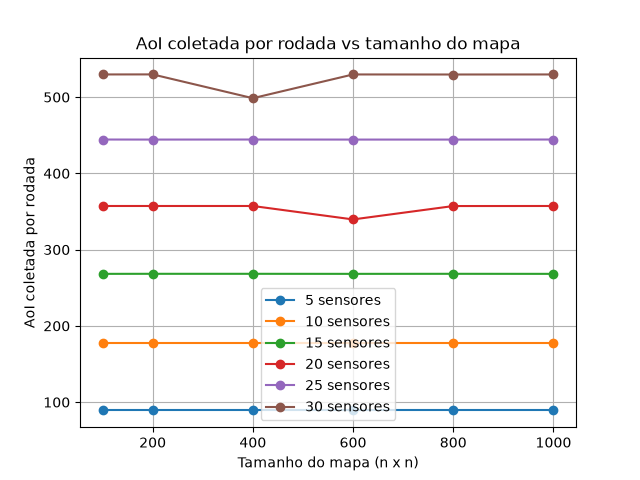
\includegraphics[width=\linewidth]{anafi_collected_aoi_vs_map.png}
    \end{column}
    \begin{column}{0.38\textwidth}
      \begin{itemize}
        \item Objetivo principal: maximizar a AoI coletada.
        \item Cresce de forma aproximadamente linear com o número de sensores.
        \item Estável em relação ao tamanho do mapa.
      \end{itemize}
    \end{column}
  \end{columns}
\end{frame}

\begin{frame}{Resultados: energia}
  \begin{columns}[c]
    \begin{column}{0.62\textwidth}
      \centering
      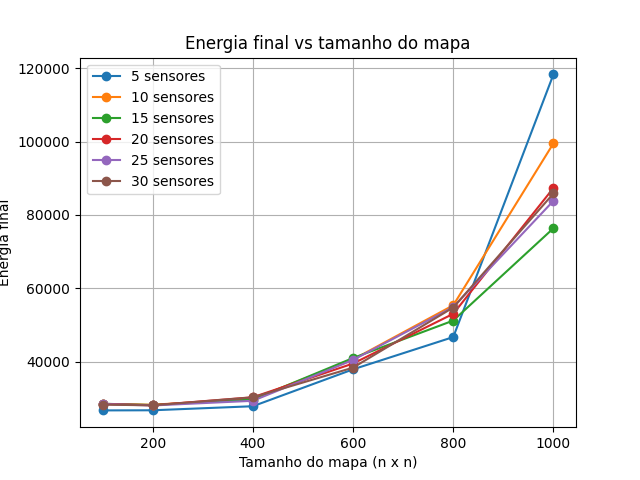
\includegraphics[width=\linewidth]{anafi_energy_vs_map.png}
    \end{column}
    \begin{column}{0.38\textwidth}
      \begin{itemize}
        \item A energia cresce com o tamanho do mapa.
        \item Maior densidade de sensores reduz distâncias e AoI.
        \item O modelo distribui as visitas de forma estável entre as rodadas.
      \end{itemize}
    \end{column}
  \end{columns}
\end{frame}

\begin{frame}{Comparação com heurísticas}
  \begin{center}
  \small
  \begin{tabular}{lrrrr}
    \toprule
    \textbf{Métrica} & \textbf{MILP} & \textbf{NN} & \textbf{AoI-G} & \textbf{Score-G} \\
    \midrule
    AoI coletada/rodada & \textbf{309,7} & 145,4 & 298,5 & 300,5 \\
    AoI média final     & \textbf{17,8}  & 127,2 & 29,5  & 28,5 \\
    Energia final (J)   & \textbf{44.943} & 48.711 & 64.571 & 57.738 \\
    Distância total (m) & 1.933 & 1.272 & 1.719 & 1.502 \\
    \bottomrule
  \end{tabular}
  \end{center}
  \vspace{0.4em}
  \begin{itemize}
    \item O MILP entrega a maior AoI coletada com o menor consumo de energia.
    \item As heurísticas por AoI ficam a $\approx 3\%$ da AoI coletada do ótimo.
    \item Score-Greedy é a melhor heurística (equilíbrio entre coleta e energia).
  \end{itemize}
\end{frame}

\begin{frame}{Variante com revisitas ($K=3$)}
  \begin{columns}[c]
    \begin{column}{0.58\textwidth}
      \centering
      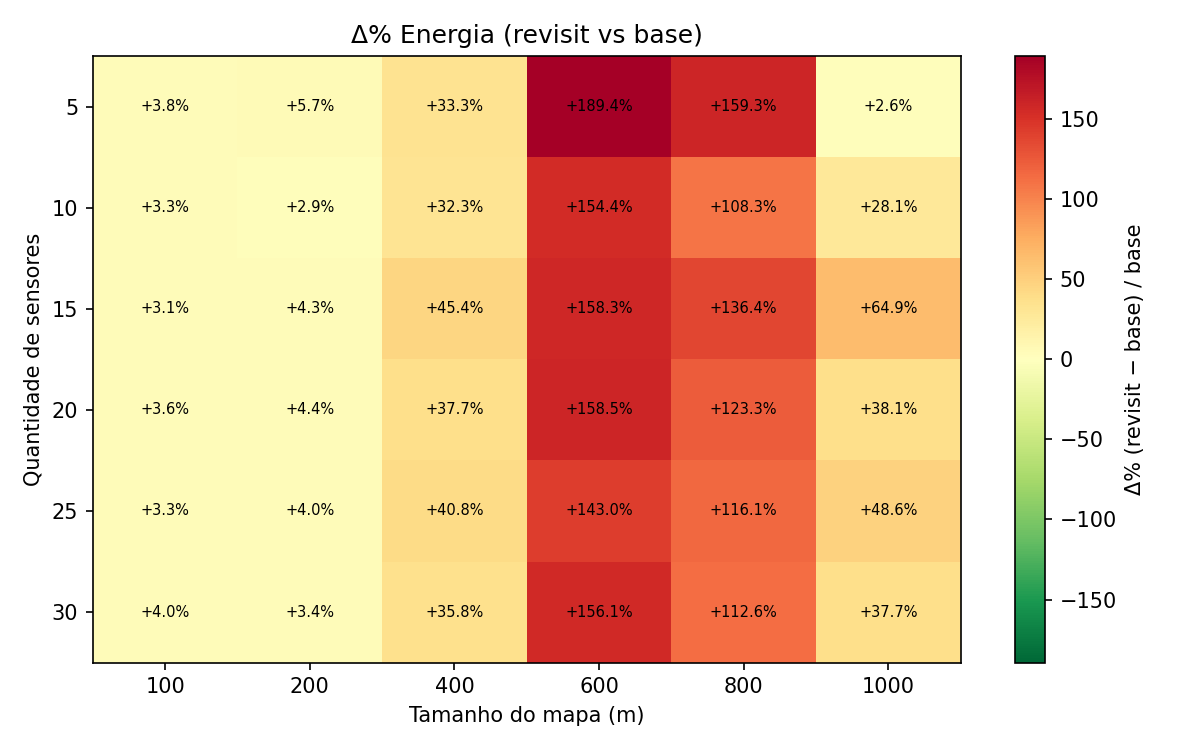
\includegraphics[width=\linewidth]{delta_energy_heatmap.png}
    \end{column}
    \begin{column}{0.42\textwidth}
      \begin{itemize}
        \item Permitir revisitar sensores \textbf{não melhora} a AoI ($\pm 3\%$).
        \item Aumenta muito a energia em mapas maiores.
        \item A restrição de \textbf{visita única} é uma escolha eficiente.
      \end{itemize}
    \end{column}
  \end{columns}
\end{frame}

\begin{frame}{Heurísticas como alternativa ao MILP}
  \begin{itemize}
    \item O modelo exato (MILP) é custoso em tempo e memória em instâncias grandes.
    \item As heurísticas executam muito mais rápido e com menos recursos.
    \item Entregam qualidade de coleta próxima à do ótimo (em especial a Score-Greedy).
    \item Alternativa prática quando o MILP se torna inviável.
  \end{itemize}
\end{frame}

\begin{frame}{Conclusões e trabalhos futuros}
  \textbf{Conclusões}
  \begin{itemize}
    \item Formulação MILP multiobjetivo lexicográfica (AoI + energia) validada em 36 cenários e dois VANTs.
    \item A restrição de visita única mostrou-se eficiente.
    \item Heurísticas (em especial Score-Greedy) aproximam o ótimo com custo muito menor.
  \end{itemize}
  \vspace{0.6em}
  \textbf{Trabalhos futuros}
  \begin{itemize}
    \item Reformulação com restrições explícitas de velocidade (desacoplar a velocidade da duração do \emph{slot}).
    \item Múltiplos VANTs cooperativos e instâncias de maior porte.
    \item Modelos de comunicação e de geração de dados mais realistas.
  \end{itemize}
\end{frame}

\begin{frame}[standout]
  Obrigado!

  \vspace{1em}
  \small Perguntas?
\end{frame}

\end{document}
